%%%%%%%%%%%%%%
% LECTURE 15 %
%%%%%%%%%%%%%%
\vspace{1cm}
\newline
\lecture{15}{26/11/2021}
\subsection{Topological quantum computing}
Nella sezione precedente abbiamo associato le eccitazioni nel sistema di spin (errori nel toric code) a due diverse tipologie di quasiparticle:  elettriche e  magnetiche. Queste quasiparticle si originano in coppia quando si verifica un bit flip o un phase flip in un qualunque punto del reticolo. Notiamo che queste quasiparticle possono essere separate all'interno del reticolo senza alcun costo in termini energetici, perché possiamo costruire un percorso generico che le colleghi attraverso l'applicazione ripetuta di X-gate (quasiparticle magnetiche) o Z-gate (quasiparticle elettriche). In Figura \ref{fig:x-equiv-lattice} è evidenziata come la posizione delle quasiparticle (magnetiche ed elettriche) all'interno dei due reticoli abbia la stessa differenza in energia $\Delta E=2J$ indipendentemente dalla loro vicinanza.

\begin{figure}[!ht]
	\centering
	\subfloat[][\label{subfig:x-nopath-lattice}]{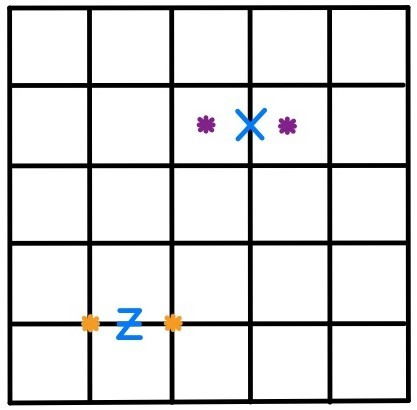
\includegraphics[scale=.5,keepaspectratio]{images/x-nopath-lattice.jpg}} \qquad \qquad
	\subfloat[][\label{subfig:x-path-lattice}]{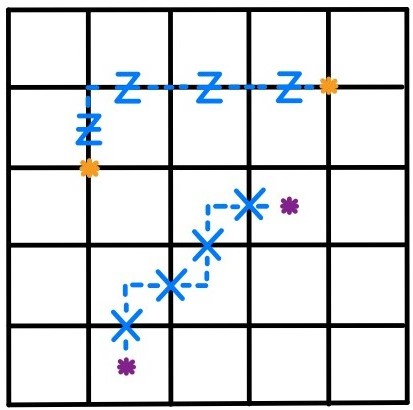
\includegraphics[scale=.5,keepaspectratio]{images/x-path-lattice.jpg}}
	\caption{(\ref{subfig:x-nopath-lattice}) Coppia di quasiparticle elettriche (asterischi arancio per $A_v = -1$) e magnetiche (asterischi viola per $B_p = -1$) create da un singolo errore. (\ref{subfig:x-path-lattice}) Indipendentemente dal cammino di errori che origina queste particelle, il costo di energia $E - E_0 = 2 J$ è sempre lo stesso.}
    \label{fig:x-equiv-lattice}
\end{figure}

\noindent In aggiunta queste quasiparticle presentano delle ulteriori proprietà interessanti. Supponiamo di considerare due coppie, una di quasiparticle elettriche e l'altra di quasiparticle magnetiche, come mostrato in Figura \ref{fig:z-path-around-x}. Immaginiamo di considerare solamente la coppia elettrica: come visto nella scorsa sottosezione, se muoviamo una delle due particelle applicando una stringa di \texttt{Z-gate} lungo un loop chiuso, allora l'effetto è banale perché il percorso può essere fattorizzato in un prodotto di operatori $B_p$, i quali hanno tutti autovalori $+1$ sul codewords. 

\noindent Il comportamento risulta tuttavia differente se consideriamo in aggiunta una coppia di particelle magnetiche. Come in figura, realizziamo un circuito chiuso (quindi tornerà nel suo punto iniziale) a partire da una particella elettrica che passi tra le due quasiparticle magnetiche. Quando il percorso va ad avvolgere una quasiparticle magnetica, siccome $X$ e $Z$ anticommutano tra loro, lo stato ottiene un termine di fase $ \ket{\psi} \to - \ket{\psi} =  e^{i\pi} \ket{\psi}$ dovuto al fatto che questa volta il prodotto di plaquette abbia autovalore $-1$. Questo risultato assomiglia un po' all'effetto Aharonov-Bohm\footnote{Dopo aver percorso un circuito chiuso torniamo allo stato iniziale con una fase extra.}: per questo motivo si dice che queste quasiparticle abbiano una statistica reciproca non banale.

\begin{figure}[!ht]
    \centering
    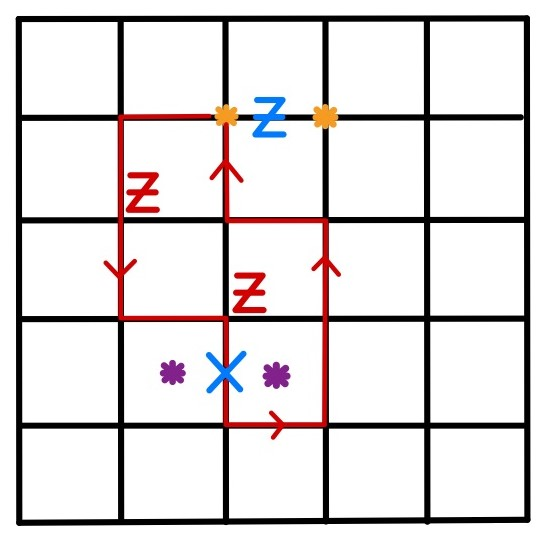
\includegraphics[scale=0.45]{images/z-path-around-x.jpg}
    \caption{Il loop chiuso di \texttt{Z-gate} (loop rosso) della quasiparticle elettrica attorno a quella magnetica produce un termine di fase a seguito di $\acomm{X}{Z} = 0$.}
    \label{fig:z-path-around-x}
\end{figure}

\noindent Riassumiamo ciò che abbiamo imparato sull'interpretazione in meccanica statistica del toric code. Questo codice di correzione degli errori presenta un approccio topologico: mentre gli errori agenti sui singoli qubit possono essere corretti similmente ai codici visti in precedenza, la situazione è differente quando si considerano errori agenti su più di un qubit simultaneamente. Immaginiamo che in un codice di protezione dagli errori come quello di Shor o di Steane avvengano 3 errori simultanei che causino $\ket{000} \to \ket{111}$. In generale, dato che un qubit logico si è trasformato in un altro qubit logico, una tale situazione è molto difficile da distinguere e correggere per quel tipo di codici. Al contrario, nel toric code, errori tali che trasformino qubit logici in altri qubit logici sono molto difficili da avere perché sono necessari degli interi loop di errori che attraversano tutto il reticolo (si pensi a $\overline{Z}_i$ e $\overline{X}_i$ della Figura \ref{fig:torus}). Se il reticolo è grande abbastanza questi errori sono molto improbabili: un reticolo sufficientemente grande assicura una protezione da questa tipologia di errori!

\noindent Dal punto di vista della sua interpretazione in meccanica statistica, questa robustezza del toric code contro gli errori si traduce in una robustezza della degenerazione dei vuoti, ossia degli stati di ground, contro le perturbazioni. Possiamo formalizzare questa proprietà nel seguente modo. Per tutti gli operatori \textit{locali}\footnote{Operatori costruiti a partire da una collezione di $X$, $Z$ e $Y$ che agiscono solo localmente in una regione finita del piano del reticolo; non sono gli operatori $\overline{Z}_i$ e $\overline{X}_i$, ossia tali che attraversino l'intero reticolo.} $\hat{O}$, chiamando $\ket{\overline{x}\overline{y}}$ e $\ket{\overline{x}'\overline{y}'}$ due differenti stati di ground, vale
\begin{equation*}
    \mel{\overline{x}\overline{y}}{\hat{O}}{\overline{x}'\overline{y}'} = \delta_{\overline{x} \overline{x}'} \delta_{\overline{y} \overline{y}'} \, , \quad \text{per} \quad \overline{x}, \overline{y}, \overline{x}', \overline{y}' = 0,1 \, .
\end{equation*}
Questo significa che operatori locali non possono tramutare stati di ground in altri stati di ground. Il motivo della precedente proprietà è il seguente: se $\hat{O}$ è locale allora è un loop di $X$ o $Z$, che agisce banalmente come identità, oppure è un singolo errore $X$ o $Z$, il quale sappiamo che genera uno stato non più facente parte del codewords. L'unico modo per ottenere qualcosa di non banale è quello di utilizzare un operatore non locale: qualsiasi perturbazione può agire solo localmente!


\noindent Il toric code è un esempio di \textbf{fase della materia con ordine topologico}. Queste sono caratterizzate da un entanglement a lungo raggio (LRE = long range entanglement, soprattutto per gli stati fondamentali) e presentano alcune proprietà comuni:
\begin{itemize}
    \item Degenerazione robusta dello stato fondamentale su varietà compatte (ad esempio un toro). Questo fatto è associato alla topologia della varietà: è molto difficile eliminare la degenerazione del ground state utilizzando perturbazioni locali;
    \item Ci sono eccitazioni  (quasiparticles elettriche e magnetiche) che presentano proprietà non locali, come ad esempio statistiche non banali. Si pensi all'effetto Aharonov-Bohm tipico di fasi topologiche della materia;
    \item La low-energy theory è in qualche modo topologica, ossia dipende unicamente dalla topologia della varietà che si sta considerando. Si tratta di una descrizione in termini di una cosiddetta \textbf{topological quantum field theory} (TQFT)\footnote{Introdotta da Edward Witten nel 1988.}. Per esempio ampiezze di processi in QM dipendono solo dalla topologia del cammino della particella e non dalla sua forma o velocità (Figura \ref{fig:qtft-equiv}).
    \begin{figure}[H]
        \centering
        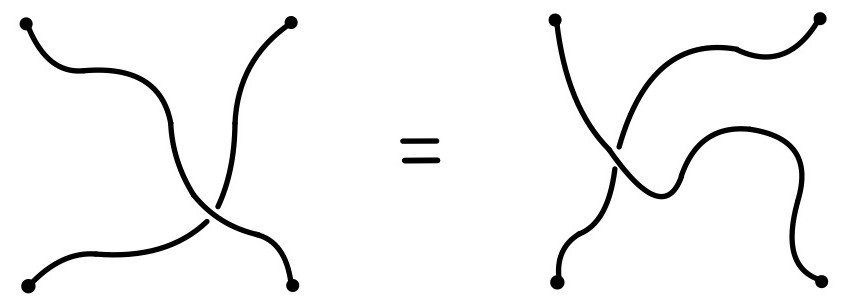
\includegraphics[scale=0.4]{images/qtft-equiv.jpg}
        \caption{Equivalenza delle ampiezze dei processi in una TQFT, i quali non dipendono dalla forma o dalla velocità dei cammini.}
        \label{fig:qtft-equiv}
    \end{figure}
\end{itemize}

\noindent Queste caratteristiche erano dal punto di vista della teoria della materia condensata. Ritornando al QC, il toric code è solitamente discusso come uno dei primi esempi di \textbf{topological quantum computing}, poiché alcune generalizzazioni di ciò che abbiamo visto nel corso di questa sezione possono essere utilizzate per il QC. Senza alcuna pretesa di essere formali, cerchiamo di comprendere quale sia l'idea che ne sta alla base. 

\noindent Dal punto di vista dell'interpretazione in meccanica statistica (sistema fisico di spin su reticolo), consideriamo l'ampiezza in QM generata dal processo in Figura \ref{subfig:circling-quasi-particles1}: se la quasiparticle elettrica circonda quella magnetica, allora, come abbiamo visto, otteniamo un termine di fase $(-1)=e^{i\pi}$ tale per cui la funzione d'onda passa da uno stato $\ket \psi$ (stato iniziale delle 4 quasiparticle) a uno stato $-\ket \psi$. Questa situazione, come mostra la Figura \ref{subfig:circling-quasi-particles2}, è assimilabile ad uno scambio di particelle: a metà del processo (linea tratteggiata in rosso in \ref{subfig:circling-quasi-particles1}) si ha una situazione in cui la particella elettrica è stata mossa nel passato di quella magnetica, quindi è come se si avesse uno scambio delle due. 

\begin{figure}[!ht]
	\centering	
	\subfloat[][\label{subfig:circling-quasi-particles1}]{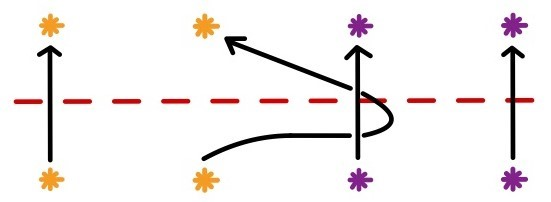
\includegraphics[scale=.4,keepaspectratio]{images/circling-quasi-particles1}} \qquad \qquad
	\subfloat[][\label{subfig:circling-quasi-particles2}]{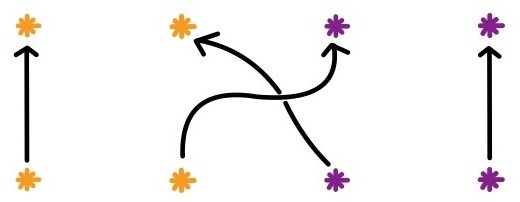
\includegraphics[scale=.4,keepaspectratio]{images/circling-quasi-particles2}}
	\caption{(\ref{subfig:circling-quasi-particles1}) Ampiezza del processo in cui una quasiparticle elettrica gira attorno ad una magnetica. (\ref{subfig:circling-quasi-particles2}) L'ampiezza qui a sinistra è analoga ad una situazione di scambio di queste particelle.}
    \label{fig:circling-quasi-particles}
\end{figure}

\noindent In una situazione di scambio di particelle dobbiamo stare attenti in QM quando si tratta di particelle identiche (si pensi alla Figura \ref{subfig:circling-quasi-particles2} con 4 particelle identiche come stato iniziale e finale): dobbiamo prestare attenzione al principio di esclusione di Pauli! 

\noindent Supponiamo di avere un sistema (in teoria della materia condensata) con un insieme di quattro\footnote{Ne consideriamo quattro perché in questi modelli le quasiparticle vengono prodotte in coppia.} quasiparticle tali per cui lo stato iniziale sia descritto dalla sovrapposizione $\ket \psi = \alpha \ket{\psi_1} + \beta \ket{\psi_2}$, la quale è degenere: ci sono due stati quantistici $\ket{\psi_1}$ e $\ket{\psi_2}$ che corrispondono alle quattro particelle identiche con i medesimi numeri quantici. Quando scambiamo due di loro come in Figura \ref{subfig:circling-quasi-particles2} avremo in generale
\begin{equation*}
    \ket \psi = \alpha \ket{\psi_1} + \beta \ket{\psi_2} \longrightarrow \ket \psi' = \alpha' \ket{\psi_1} + \beta' \ket{\psi_2} \, .
\end{equation*}
La relazione che lega questo scambio può essere vista come una rotazione non banale operata dalla matrice unitaria $\hat{U}$:
\begin{equation*}
    \begin{pmatrix}
        \alpha \\
        \beta
    \end{pmatrix}
    \longrightarrow
    \begin{pmatrix}
        \alpha' \\
        \beta'
    \end{pmatrix}
    =\hat U
    \begin{pmatrix}
        \alpha \\
        \beta
    \end{pmatrix} \, ;
\end{equation*}
in particolare ritorniamo alla condizione iniziale, ma con lo stato che può essere trasformato in un altro stato dello stesso spazio di Hilbert degenere. L'unico vincolo quantomeccanico è il fatto che $\hat U$ sia unitario. 

\noindent Questi stati presentano quella che si definisce \textbf{statistica non-abeliana} (il toric code ha solo uno stato per cui la statistica era abeliana, ossia data da una semplice fase del gruppo $U(1)$). Quando le particelle sono identiche e presentano statistica frazionaria, allora, non essendo né fermioni né bosoni, sono note come \textbf{anyons} e possono esistere solamente in una situazione bidimensionale\footnote{Non nello spazio tridimensionale, perché in 3D un doppio scambio deve essere banale per via della topologia, cosicché un singolo scambio possa dare solo $\pm1$ (bosoni o fermioni).}. 

\noindent La cosa curiosa è che, in teoria, gli anyons non-abeliani possono essere usati per il QC! Costruendo in laboratorio un array di quasiparticle e intrecciandole tra loro possiamo dare luogo a trasformazioni unitarie non-abeliane proprio come l'esempio di Figura \ref{fig:tqc}. Ogni volta che si scambia una quasiparticle si ha una trasformazione unitaria sul sistema: l'intera sequenza di scambi può essere pensata come un singolo operatore (gate) unitario $U$.

\begin{figure}[!t]
    \centering
    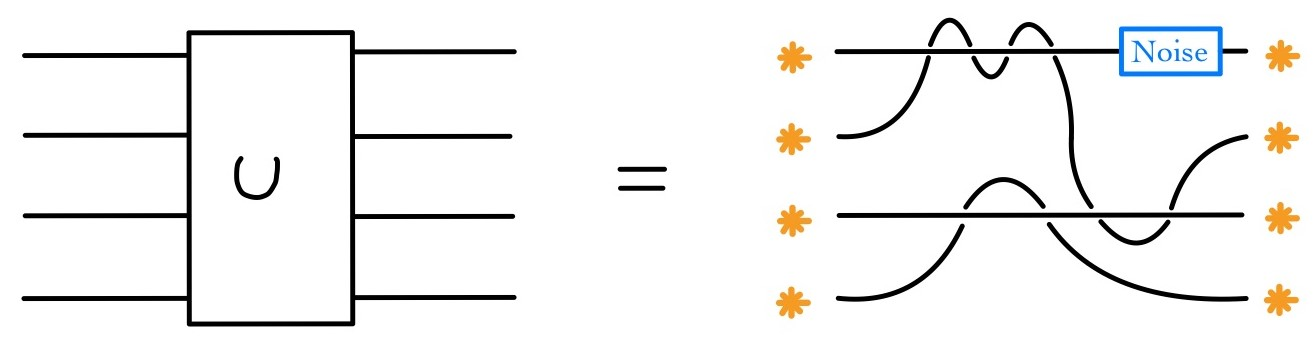
\includegraphics[scale=0.4]{images/tqc.jpeg}
    \caption{Implementazione in QC di un circuito utilizzando un array di quasiparticle. Si suppone che i fili del circuito possano essere sostituiti dalle particelle, le quali possono essere spostate tra loro. Il rumore può intervenire unicamente su un singolo intreccio: per cambiare l'intero $U$ dovrebbe annullare ogni singolo intreccio!}
    \label{fig:tqc}
\end{figure}

\noindent Se fossimo in grado di realizzare abbastanza trasformazioni unitarie con scambi multipli, potremmo eseguire del QC grazie ad essi. Perché sarebbe molto interessante poter costruire computer quantistici basati su questo funzionamento? Questi dispositivi sarebbero molto robusti e fault-tolerant perché il rumore o altri disturbi locali andrebbero ad agire solo localmente sulla linea delle quasiparticle. Affinché il disturbo causato dall'ambiente possa essere in grado di cambiare l'intero $U$, esso dovrebbe poter annullare tutte le singole trasformazioni.

\noindent I tipi più comuni di anyons (non-abeliani) sono:
\begin{itemize}
    \item \textbf{Ising Anyons}: non sono universali nel senso del QC, ma appaiono teoreticamente in molti sistemi della materia condensata:
        \begin{itemize}
            \item Effetto Hall quantistico frazionario ($\nu=5/2$; SU(2)$_2$ nel contesto della TQFT);
            \item Majorana zero-mode in superconduttori topologici bidimensionali (generalizzano il più semplice modello monodimensionale chiamato catena di Kitaev).
        \end{itemize}
    \item \textbf{Fibonacci Anyons}: sono universali, sono stati sviluppati nella teoria dei modelli che generalizzano il toric code e si suppone che appaiano nell'effetto Hall quantistico frazionario ($\nu=12/5$; SU(2)$_3$ nel contesto della TQFT).
\end{itemize}
Due figure di spicco che proposero e diedero inizio al campo del topological quantum computing sono:
\begin{itemize}
    \item Alexei Kitaev, il quale propose nel 1997 un topological quantum computing basato sugli anyons;
    \item Michael Freedman, vincitore nel 1986 della medaglia Fields per aver risolto la congettura di Poincaré in dimensione 4. Era interessato a calcolare degli invarianti della teoria dei nodi noti come polinomi di Jones,  un problema di difficoltà esponenziale dal punto di vista del CC, quando scoprì che in QC in realtà può essere risolto in un tempo polinomiale. Attualmente dirige il gruppo di Microsoft Station Q a Santa Barbara per lo sviluppo del topological quantum computing. Nel 2018 il gruppo annunciò di aver realizzato sperimentalmente i Majorana zero-mode, ma nel 2021 l'articolo fu ritirato.
\end{itemize}






\chapter{Realizzazione fisica dei qubit}

\section{Introduzione}
Nella parte introduttiva del primo capitolo abbiamo visto che esistono moltissimi modi per poter realizzare fisicamente un qubit, dato che, dal punto di vista della QM, si tratta di un qualsiasi sistema quantistico a due livelli. Lasciando stare il discorso sulla realizzazione dei qubit nell'ambito della topological quantum computing, i più semplici da realizzare sono basati su:
\begin{itemize}
    \item Sistemi costituiti da particelle con \textbf{Spin} $1/2$; le particelle possono essere semplicemente controllate attraverso un campo magnetico $\vec B$, in quanto l'hamiltoniana che descrive questo tipo di interazione con lo spin è
    \begin{equation*}
        \hat H = - \mu \hat{\vec S} \cdot \vec B \, ,
    \end{equation*}
    dove $\mu$ è il momento magnetico.
    
    \item Sistemi che sfruttano la \textbf{polarizzazione dei fotoni}; sono in generale più difficili da gestire rispetto ai precedenti, tuttavia possono essere opportunamente controllati attraverso filtri polarizzatori (ad esempio un prisma per controllare i cambi di fase), beam splitters, ecc.
\end{itemize}

\noindent Altre realizzazioni fisiche, alcune delle quali approfondiremo nelle prossime sezioni, riguardano i qubit superconduttivi\footnote{Utilizzati da IBM e Google.}, i qubit basati sulla risonanza magnetica nucleare\footnote{Nota meglio come NMRQC: Nuclear Magnetic Resonance Quantum Computing.}, i qubit a trappola ionica\footnote{Utilizzata da IonQ.}, ecc. Spendiamo alcune parole sui qubit realizzati mediante sistemi basati sulla trappola ionica e sulla superconduttività. 

\noindent Nei primi dispositivi si vuole andare a creare un campo elettromagnetico che confini un insieme di ioni in una catena lineare lungo una direzione privilegiata (per convenzione è l'asse $z$). Si veda la Figura \ref{fig:ion-trap1} per una raffigurazione schematica. 

\begin{figure}[!t]
    \centering
    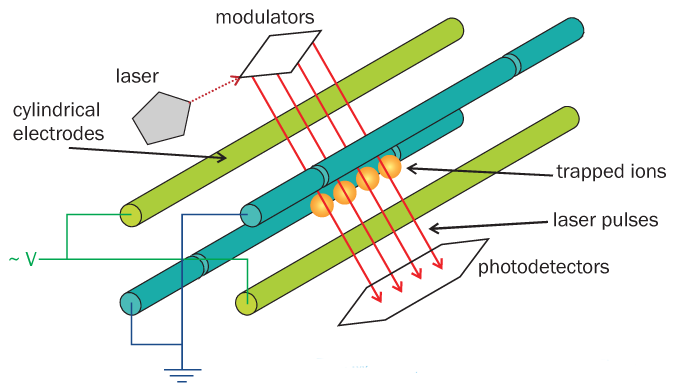
\includegraphics[scale=0.5]{images/ion-trap1}
    \caption{Rappresentazione schematica del sistema della trappola ionica.}
    \label{fig:ion-trap1}
\end{figure}

\noindent L'idea è quella di raffreddare questo sistema fino allo stato fondamentale in maniera tale che l'unico grado di libertà rimanente a questi ioni riguardi piccole vibrazioni lungo l'asse z. In questo modo si può incorporare un qubit in ognuno di essi combinando due differenti tipi di sistemi a due livelli:
\begin{itemize}
    \item Ogni ione presenta una struttura iperfine nei livelli energetici, si avrà quindi uno stato fondamentale $\ket 0$ e uno stato eccitato $\ket 1$, il quale è metastabile. Essi sono separati da un'energia pari a $\hbar\omega_1$.
    
    \item Ogni ione ha però al tempo stesso un modo vibrazionale, il quale è assimilabile a un oscillatore armonico. In termini di fisica della materia condensata, ogni \textbf{fonone} ha quindi due stati energetici separati da un'energia pari a $\hbar\omega_2$.
\end{itemize}

\noindent Perciò è possibile costruire due qubit identificando lo stato con la notazione $\ket{nm}$, dove $n$ indica il primo sistema a due livelli (livelli iperfini dello ione) ed $m$ il secondo sistema a due livelli (modi del fonone), proprio come mostrato in Figura \ref{fig:ion-trap2}. Utilizzando infine degli impulsi generati da laser, si può andare a interagire e a manipolare questo sistema (si pensi alla Figura \ref{fig:ion-trap1}).

\begin{figure}[!ht]
    \centering
    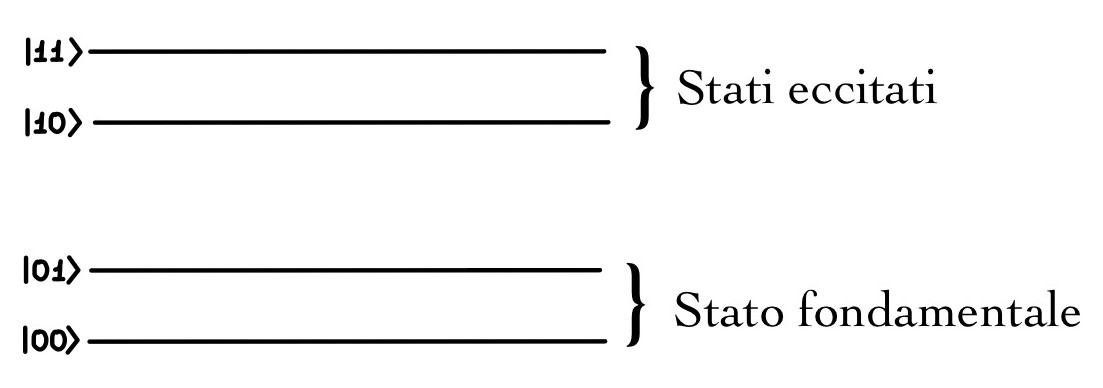
\includegraphics[scale=0.45]{images/ion-trap2.jpg}
    \caption{Sistema doppio a due livelli che coinvolge gli stati energetici degli ioni e i modi vibrazionali dei fononi. Notare che la differenza energetica tra gli stati fondamentali e gli stati eccitati è maggiore rispetto alla differenza energetica dovuta ai modi vibrazionali.}
    \label{fig:ion-trap2}
\end{figure}

\noindent Per quanto riguarda invece i sistemi superconduttivi l'idea che sta alla base è quella di realizzare un semplice circuito LC.  Risolvendo le equazioni di Kirchhoff è possibile mostrare che il comportamento di tale circuito sia quello di un oscillatore armonico, il quale può essere facilmente quantizzato attraverso la quantizzazione canonica. Si parla di superconduttività poiché si cerca di lavorare con elementi che non presentano alcuna resistenza a bassa temperatura. 

\noindent Il problema, che ribadiremo più volte, è che questo circuito LC per come è fatto non è molto adatto a descrivere un sistema a due livelli, dunque bisogna fare in modo che il comportamento dell'oscillatore risulti anarmonico: solitamente lo si fa introducendo la cosiddetta \textbf{giunzione Josephson}, per mezzo della quale si passa da un sistema a livelli equispaziati a un sistema con livelli non più equidistanti e che presentano dell'anarmonicità. Per interagire con questi sistemi è poi quindi necessario introdurre un generatore di impulsi a microonde mentre per ottenere informazioni sui qubit si utilizzano delle cavità elettromagnetiche. La differenza sostanziale tra i due dispositivi sta nel campo elettromagnetico, in quanto nel primo è classico mentre nel secondo è quantizzato. Si veda la Figura \ref{fig:lc-circuit-cavity} per una rappresentazione schematica.

\begin{figure}[!ht]
    \centering
    \begin{circuitikz}
        \draw
        (0,0)   to[C=$C$] ++ (0, 2) -- ++ ( 2,0) 
                to[L=$L$] ++ (0,-2) -- ++ (-2,0)
        %
        (0.5,2) |- ++ (-1.5,0.5) node[left, draw] {V(t)}
        (1.5,2) |- ++ ( 1.5,0.5) node[right,draw, align=center] {E.M.\\ Cavity};
    \end{circuitikz}
    \caption{Circuito LC con generatore di microonde e cavità elettromagnetica.}
    \label{fig:lc-circuit-cavity}
\end{figure}


\section{Oscillatore armonico quantistico}
Prima di poter descrivere accuratamente un modello fisico completo per un computer quantistico realizzabile, richiamiamo alcune nozioni su un sistema fisico molto elementare: l'oscillatore armonico quantistico\footnote{Non ci dilunghiamo molto su questo argomento perché è stato già trattato in maniera sufficientemente approfondita nel corso di MQ.}.
\noindent Supponiamo di avere un sistema che oscilla con una frequenza pari a $\omega$. Il suo moto sarà descritto dall'equazione del moto 
\begin{equation}\label{EOM_HO}
    \dv[2]{x}{t} + \omega^2 x = 0 \, ,
\end{equation}
le cui soluzioni sono del tipo $x(t) = e^{\pm i \omega t}$. L'hamiltoniana associata a questo sistema risulta quindi in
\begin{equation}\label{eq:ham-oa}
    H = \frac{p^2}{2m}+ \frac 12 m \omega^2 x^2 \, .
\end{equation}
Per passare ad una descrizione quantomeccanica si procede  con la quantizzazione canonica identificando le osservabili posizione e momento lineare con i rispettivi operatori hermitiani $\hat x$ e $\hat p$; inoltre introduciamo la regola di commutazione $\comm{\hat x}{\hat p}=i\hbar$. In questo modo l'hamiltoniana \eqref{eq:ham-oa} può essere scritta immediatamente come
\begin{equation*}
    \hat H = \frac{\hat p ^2}{2m} + \frac 12 m\omega^2 \hat x^2 \, ,
\end{equation*}
oppure
\begin{equation}\label{eq:ham-oa2}
    \hat H = \hbar \omega\left(\hat a^\dagger \hat a+\frac 12\right)=\hbar \omega\left(\hat n +\frac 12\right) \, ,
\end{equation}
dove in quest'ultima equazione abbiamo introdotto tre nuovi operatori
\begin{align*}
    &\text{Operatore di creazione:} &\hat a^\dagger &= \frac{1}{\sqrt{2m\hbar \omega}}(m\omega \hat x - i\hat p) \, , \\
    &\text{Operatore di distruzione:} &\hat a &= \frac{1}{\sqrt{2m\hbar \omega}}(m\omega \hat x + i\hat p) \, , \\
    &\text{Operatore numero:} &\hat n &= \hat a^\dagger \hat a \, .
\end{align*}
Dalla relazione di commutazione precedente avremo $\comm{a}{a^\dagger}=1$. Con queste definizioni, possiamo anche riscrivere $\hat x$ e $\hat p$ in funzione dei primi due nuovi operatori
\begin{align}
    \hat x &= \sqrt{\frac{\hbar}{2m\omega}}\left(\hat a + \hat a^\dagger\right) \, , \label{x_a_adag} \\
    \hat p &= -i\sqrt{\frac{m\omega\hbar}{2}}\left(\hat a - \hat a^\dagger\right) \, .
\end{align}
Con queste nuove definizioni avremo che gli autostati dell'hamiltoniana \eqref{eq:ham-oa2} sono gli stessi dell'operatore numero $\hat n$, quindi possiamo considerare una base comune di autostati $\ket n$ tale per cui $\hat n \ket n = n \ket n$. Esplicitamente avremo
\begin{equation*}
    \hat H \ket n = \hbar \omega \left(n + \frac 12 \right)\ket n \, , \quad \text{dove} \quad n \in \mathbb{N} \, .
\end{equation*}
La cosa importante da sottolineare è che gli operatori $\hat a^\dagger$ e $\hat a$ non a caso sono chiamati operatori di creazione e distruzione, perché a partire dallo stato fondamentale $\ket 0$, che ha energia $\frac{\hbar\omega}{2}$, possiamo costruire tutti gli altri livelli. L'azione su un autostato $\ket n$ non è altro che
\begin{equation}\label{a_adag_action_states}
\begin{aligned}
    &\hat a^\dagger \ket n = \sqrt{n+1}\ket{n+1}\, , \\
    &\hat a \ket n = \sqrt n \ket{n-1} \, .
\end{aligned}
\end{equation}
Pertanto, per costruire il livello $n$-esimo, sarà sufficiente applicare la definizione sul ground state $\ket{0}$:
\begin{equation*}
    \ket n = \frac{(a^\dagger)^n}{\sqrt{n!}}\ket 0 \, .
\end{equation*}
Se ora andassimo a rappresentare graficamente il potenziale armonico
\begin{equation*}
    V(x) = \frac 12 m \omega^2 x^2 \, ,
\end{equation*}
con le varie funzioni d'onda (\textit{polinomi di Hermite}), potremmo osservare l'andamento rappresentato in Figura \ref{fig:qha}. Dal momento che tutti i livelli sono equispaziati, ciascun livello differisce dal precedente e dal successivo per un termine $\hbar\omega$: l'idea, per realizzare un sistema a due livelli, è quindi quella di considerare i livelli $n=0$ e $n=1$, che identifichiamo con $\ket 0$ e $\ket 1$, come stati del nostro qubit. Allo stesso tempo però dobbiamo essere in grado di controllare il passaggio dallo stato fondamentale $\ket 0$ allo stato eccitato $\ket 1$ e questo può essere facilmente realizzato attraverso un impulso laser. Tuttavia è possibile che il nostro sistema si trovi già in uno stato eccitato e mediante un altro impulso laser passi a un livello eccitato che si trova al di fuori del nostro sistema a due livelli, ad esempio si può verificare
\begin{align*}
    \ket{1} &\longrightarrow \ket{2} \, , \\
    \ket{2} &\longrightarrow \ket{3} \, , \\
    \vdots \; &\longrightarrow \; \vdots
\end{align*}
Per cui la descrizione dell'oscillatore armonico quantistico è sì utile per la realizzazione di sistemi a due livelli, però presenta dei difetti correlati al fatto che i livelli energetici siano equidistanti. Vedremo nelle sezioni successive come si può intervenire per ovviare a questo inconveniente.

\noindent Sebbene quest'ultimo aspetto sia spesso visto come un problema per la realizzazione di un qubit, l'oscillatore armonico quantistico può essere utilizzato per realizzare alcuni gate non banali. Vediamo il seguente esempio accademico.

\begin{figure}[!t]
    \centering
    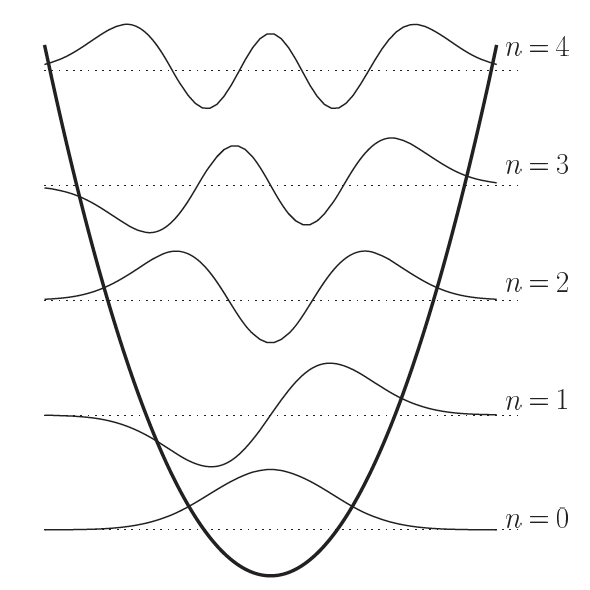
\includegraphics[scale=0.6]{images/qho.png}
    \caption{Potenziale armonico con le funzioni d'onda associate. I livelli energetici sono chiaramente equidistanti dal punto di vista energetico, quindi è molto difficile interagire con dei livelli a piacere mediante l'utilizzo della radiazione.}
    \label{fig:qha}
\end{figure}

\begin{esempio}[\textbf{Codifica del CNOT gate.}]
    Supponiamo di voler eseguire un calcolo quantistico che faccia uso di un \texttt{CNOT-gate} costruito con l'oscillatore armonico quantistico descritto sopra. Che cosa possiamo fare? La scelta più naturale per la rappresentazione dei qubit sono gli autostati energetici $\ket n$. Questa scelta ci permette di eseguire un \texttt{CNOT-gate} nel seguente modo: codifichiamo i seguenti 4 qubit logici utilizzando l'identificazione
    \begin{equation}\label{eq:cnot-qho}
        \begin{aligned}
            \ket{00}_L &= \ket{0} \, , &\ket{01}_L &= \ket{2} \, ,\\
            \ket{10}_L &= \frac{\ket{4}+\ket{1}}{\sqrt 2} \, , &\ket{11}_L &= \frac{\ket{4}-\ket{1}}{\sqrt 2} \, ,
        \end{aligned}
    \end{equation}
    \noindent dove il pedice $L$ è usato per distinguere chiaramente gli stati logici in contrasto con gli autostati dell'hamiltoniana dell'oscillatore armonico. Dal punto di vista concettuale, il fatto che stiamo utilizzando stati energetici come $\ket 2$ e $\ket 4$ sarà presto chiaro.
    
    \noindent La manipolazione dei qubit, come abbiamo visto all'inizio, può essere effettuata, ad esempio, tramite l'applicazione di un campo magnetico nel caso di un sistema con degli spin: in generale può essere necessario sottoporre il sistema a delle perturbazioni esterne. In questo caso possiamo semplicemente sfruttare l'evoluzione temporale degli stati: assumiamo di aver preparato il sistema in uno stato $\ket{n}$ e decidiamo di lasciarlo evolvere nel tempo, quindi
    \begin{equation*}
        \ket n \rightarrow \hat{U}(t) \ket{n} =  e^{-\frac{i}{\hbar}\hat{H} t} \ket{n} = e^{-\frac{i}{\hbar} E_n t} \ket{n} \, ;
    \end{equation*}
    lo stato finale rimane nello stato di partenza acquisendo tuttavia una fase: il punto importante che ci permette di costruire un \texttt{CNOT-gate} è che l'evoluzione temporale non crea una sovrapposizione di stati, ma mantiene bensì un singolo stato stazionario. Ricordando che i livelli energetici sono dati da
    \begin{equation*}
        E_n = \hbar \omega \left(n+\frac 12\right) \, ,
    \end{equation*}
    allora, trascurando il fattore $1/2$ perché fase comune a tutti i livelli, possiamo procedere nell'applicare l'operatore di evoluzione temporale agli stati logici in \eqref{eq:cnot-qho}
    \begin{align*}
        \ket{00}_L &= \ket{0} \, , &\ket{01}_L &= e^{-2i\omega t}\ket{2} \, , \\
        \ket{10}_L &= \frac{e^{-4i\omega t}\ket{4}+e^{-i\omega t}\ket{1}}{\sqrt 2} \, , &\ket{11}_L &= \frac{e^{-4i\omega t}\ket{4}-e^{-i\omega t}\ket{1}}{\sqrt 2} \, .
    \end{align*}
    Se scegliamo un valore di tempo particolare, come ad esempio $t=\pi/\omega$, l'evoluzione temporale porterà allora a
    \begin{align*}
        \ket{00}_L &\rightarrow \ket{0} \equiv \ket{00}_L \, , &\ket{01}_L &\rightarrow \ket{2} \equiv \ket{01}_L \, , \\
        \ket{10}_L &\rightarrow \frac{\ket{4}-\ket{1}}{\sqrt 2} \equiv \ket{11}_L \, , &\ket{11}_L &\rightarrow \frac{\ket{4}+\ket{1}}{\sqrt 2} \equiv \ket{10}_L \, \, .
    \end{align*}
    Abbiamo ottenuto esattamente l'azione di un \texttt{CNOT-gate} utilizzando semplicemente l'evoluzione temporale del sistema!
\end{esempio}

\noindent Perché non è possibile utilizzare fisicamente un \texttt{CNOT-gate} così costruito? Perché ogni conto in QC è basato sul calcolo quantistico, non sul calcolo analogico: per usare i qubit ottenuti è necessario intervenire mediante l'utilizzo della radiazione, ma così ritorniamo al problema originale dei livelli energetici equispaziati! È semplice costruire un \texttt{CNOT-gate}, ma purtroppo è molto difficile controllare un tale sistema.  

